%% Used the following Template:
%
%% This is file `PatentApplication.tex',
%% 
%% 
%%   Author: Peter J. Pupalaikis  (pete_pope  at hotmail dot com)
%%   Copyright 2012 Peter J. Pupalaikis
%%   Version 1.0
%% 
%%   This work may be distributed and/or modified under the
%%   conditions of the LaTeX Project Public License, either
%%   version 1.3 of this license or (at your option) any
%%   later version.
%%   The latest version of the license is in
%%      http://www.latex-project.org/lppl.txt
%%   and version 1.3 or later is part of all distributions of
%%   LaTeX version 2003/06/01 or later.
%% 
%%   This work consists of the files listed in the README file.
%% 
\documentclass[english]{uspatent}
\usepackage{graphicx}
\graphicspath{ {images/} }
\begin{document}

\setDocketNumber{Docket Number #880080}
\setLawyerName{Patent Laywer: Pat Law}
\setLawyerNumber{(925) 123-4567}
\setLawyerPhone{Patent Lawyer Phone}
\setDocumentVersion{0.0}
\setPrintingModeApplication

\include{Drawings}

\title{Stainless Steel Heat Medium Thermos}
\date{2/28/2018}
\inventor{Dailon Dolojan}

\maketitle

\patentSection{Abstract}
A double layered stainless steel thermos that utilizes an outer container, heat medium, and inner container to fully insulate and maintain the temperature of a liquid. The outer and inner container walls are made up of a double-layered stainless steel that creates a vacuum to provide insulation from external forces. The inner container will screw into the base of the outer container whereupon the heat medium will be poured or placed in between the walls of the outer container and inner container. The heat medium used can either be boiling water or a molded ice cylinder. The liquid will then be poured into the inner container where a stainless steel lid will secure and lock both containers into place. The lid will have a rectangular siphon which the user can then drink the liquid from the inner container.

\patentSection{Field of the Invention}

This invention aims to innovate the insulated water bottle and thermos industry. This invention serves a dual purpose of insulating both cold and hot drinks by further developing the structure of thermal insulation with three layers. In particular, the invention will innovate the structure of creating layers of insulation for a beverage through double layered stainless steel technology and usage of a heat medium.

\patentSection{Prior Arts}

Insulated water bottles and thermos are typically made similar to a cup-like container where the walls of the bottle are made of a double layer of stainless steel to provide insulation. The container is made of an initial layer of stainless steel that serves as the outer wall. The second layer of stainless steel is then placed and sealed on top of the initial layer of stainless steel to form a vacuum. This vacuum created by the double layer of stainless steel serves as the only insulation that is used to prevent heat transfer. Although a vacuum serves as the best form of thermal insulation, most water bottles and thermos use only one layer of insulation with top brand water bottles implementing two layers of insulation. The usage of two layers of insulation provides a significant boost in insulation of a hot or cold beverage in comparison to one layer. However, as time progresses, heat transfer will eventually occur through conduction as the container is exposed to differing temperatures. The temperature of the liquid will then begin to transfer heat energy from its environment with no internal mechanism of maintaining the temperature.
Through using another heat medium to preserve temperature, in addition to the insulated layers of the container, the temperature of the liquid can be conserved for a longer duration of time. A medium such as boiling water or ice can allow a drink to stay warm or cold longer, respectively, in conjunction with the insulated layering of the stainless steel double layering. By having another heat medium to conserve heat energy, the duration a drink stays warm or cold can be prolonged as the thermal energy of the liquid must first stabilize between the insulated layer separating the beverage and the medium. This will allow for heat transfer to be thoroughly slowed. 

\patentSection{Description of the Invention}

\hspace*{0.5cm} The main object of this invention is to create a thermos that utilizes two containers made of double layered stainless steel walls where one container will hold a medium that will mold to surround the second container that contains the liquid.
\\
\hspace*{0.5cm} The invention will utilize compact and ergonomic design to provide easy usage and effective insulation in a cylindrical shape.
\\
\hspace*{0.5cm} The complete construction of an assembled thermos is outlined in \textbf{Figure 1} where the double layered stainless steel outer container \textbf{1}, double layered stainless steel inner container \textbf{2}, and stainless steel lid \textbf{3} are properly secured and locked into place.
\\
\hspace*{0.5cm} The thermos first contains a double layered stainless steel outer container which is structured in \textbf{Figure 5}. The outer container \textbf{1} has a rim which contains metal grooves \textbf{12} for the lid as shown in \textbf{Figure 3} can screw into. Within the middle of the outer container, there is a line titled ``FILL" \textbf{13} which will indicate the amount of boiling water to pour to fill the outer container \textbf{1} completely without causing the outer container \textbf{1} to overfill. At the bottom of the base of the outer container shown in \textbf{Figure 4}, there is a segmented circular groove \textbf{11} where the inner container shown in \textbf{Figure 6} can screw into. The segmented nodules \textbf{5} will then secure the inner container \textbf{2} in place to prevent the inner container from accidentally loosening.
\\
\hspace*{0.5cm} When the inner container \textbf{2} is successfully screwed into the base of outer container \textbf{Figure 4}, the user can pour boiling water into the empty space \textbf{16} between the outer container \textbf{1} and inner container \textbf{2} to serve as a heat medium to prevent the loss of heat to a warm liquid.  The user can also use the ice mold as shown in \textbf{Figure 2} in place of the boiling water to keep liquids cold. The ice mold \textbf{Figure 2} contains a cylindrical cavity \textbf{18} where water can be poured into and then placed into a freezer to create a cylindrical ice cube. The ice mold \textbf{Figure 2} is comprised of an outer plastic cylindrical structure \textbf{10}  that will hold the water and a center rod \textbf{9} is used to form the cavity needed for the ice to fit around the inner container \textbf{2} . The ice cylinder can then be slid into the empty space \textbf{16} between the outer container \textbf{1} and inner container \textbf{2}.
\\
\hspace*{0.5cm} Once the heat medium is added to the container, the liquid can be poured into the empty space of the inner container \textbf{17}. The lid shown in \textbf{Figure 3} can then be screwed onto the outer container \textbf{1} and inner container \textbf{2} using the metal grooves of the lid \textbf{8} and the metal grooves of the outer container \textbf{12}. The lid's segmented nodules \textbf{6} will then keep the inner container \textbf{2} secured into place. The user can then drink the liquid from the inner container \textbf{2} through the foldable siphon \textbf{4}. 
\\
\hspace*{0.5cm} Within \textbf{Figure 7}, a close up of the double layered stainless steel walls that comprise to make up the wall of the outer container. The stainless steel walls \textbf{14} enclose the container in order to form a vacuum \textbf{15}. This allows for high thermal insulating properties between the outer container \textbf{1} and medium as well as the medium and inner container \textbf{2}.

\patentSection{Brief Description of Drawings}
\hspace*{0.5cm} The drawings depict various features and mechanics of the invention broken down into several figures.
\\ \hspace*{0.5cm} Within the drawings:
\\ \hspace*{1.5cm} \textbf{Figure 1.} is a sectional side view of the completed invention with the lid \\\hspace*{2.0cm} and inner container attached to the outer container.
\\ \hspace*{1.5cm} \textbf{Figure 2.} is side view of the ice mold that will be used to create the \\\hspace*{2.0cm} cylindrical ice block that will be utilized as a heat medium to further \\\hspace*{2.0cm} prevent heat transfer.
\\ \hspace*{1.5cm} \textbf{Figure 3.} is a top view of the lid that will attach the inner container and \\\hspace*{2.0cm} outer container as well as seal the liquid and medium within the bottle.
\\ \hspace*{1.5cm} \textbf{Figure 4.} is a close up of the base of the bottom of the outer container \\\hspace*{2.0cm} which contains the mechanism of how the inner container will screw into \\\hspace*{2.0cm} the base.
\\ \hspace*{1.5cm} \textbf{Figure 5.}  is a sectional view of the outer container.
\\ \hspace*{1.5cm} \textbf{Figure 6.} is a sectional view of the inner container.
\\ \hspace*{1.5cm} \textbf{Figure 7.} is a close up of the double stainless steel layer insulation used in \\\hspace*{2.0cm} the outer container 

\patentClaimsStart

\beginClaim{Claim1}

A thermos apparatus to be used by a user which is comprised of:
\\ \hspace*{0.5cm} A double layered stainless steel outer container to contain a heat medium.
\\ \hspace*{0.5cm} A double layered stainless steel inner container to contain the liquid desired \\\hspace*{1.5cm}to keep warm or cold which will attach to the outer container.
\\ \hspace*{0.5cm} A plastic cylindrical mold to create a hollowed ice cylinder which will be \\\hspace*{1.5cm}placed within the outer container and surround the inner container.
\\ \hspace*{0.5cm} A stainless steel lid that will seal and lock the double layered stainless steel \\\hspace*{1.5cm}outer and inner container into place, and a drinking mechanism to \\\hspace*{1.5cm}transfer liquid from the inner container to the user`s mouth.

\beginClaim{Claim2}

A thermos apparatus as recited in \claimRef{Claim1}, wherein the double layered stainless steel layering will be made of an exterior wall of stainless steel which is then enclosed by an interior wall of stainless steel to form a vacuum between the space separating the two walls.

\beginClaim{Claim3}

A thermos apparatus as recited in \claimRef{Claim1}, wherein the double layered stainless steel outer container will contain mechanical grooves and nodules on the inner bottom base of the container to lock the double layered stainless steel inner container in place while holding the heat medium.

\beginClaim{Claim4}

A thermos apparatus as recited in \claimRef{Claim3}, wherein the double layered stainless steel outer container will have a designated marked line to indicate the amount of boiling water to be poured into the double layered stainless steel outer container to  provide sufficient heat medium to fill the container.

\beginClaim{Claim5}

 A thermos apparatus as recited in \claimRef{Claim1}, wherein the double layered stainless steel outer container will have mechanical grooves and nodules outlining the top rim of the container to attach to the stainless steel lid.

\beginClaim{Claim6}

A thermos apparatus as recited in \claimRef{Claim1}, wherein the plastic mold will be a cylindrical case that is shaped as a mold for a cup such that liquid may be poured into the outlined mold to produce an ice block shaped like a hollow cylinder which will then be placed within the double layered stainless steel outer container.

\beginClaim{Claim7}

 A thermos apparatus as recited in \claimRef{Claim1}, wherein the double layered stainless steel inner container will have a base that has mechanical grooves and nodules that can attach to the bottom base of the double layered stainless steel outer container.

\beginClaim{Claim8}

A thermos apparatus as recited in \claimRef{Claim1}, wherein the double layered stainless steel inner container will have mechanical grooves and nodules outlining the top rim of the container to attach to the stainless steel lid.

\beginClaim{Claim9}

A thermos apparatus as recited in \claimRef{Claim1}, wherein the stainless steel lid will contain a drinking mechanism that is comprised of a folding rectangular straw that will allow for the safe transfer of both hot or cold liquids from the inner container.

\beginClaim{Claim10}

A thermos apparatus as recited in \claimRef{Claim1}, \claimRef{Claim5}, and \claimRef{Claim8}; wherein the stainless steel lid will contain mechanical grooves and nodules on its underside in order to seal the double layered stainless steel inner container with the double layered stainless steel outer container in place.

\patentClaimsEnd

\patentSection{Drawings}
\begin{center}
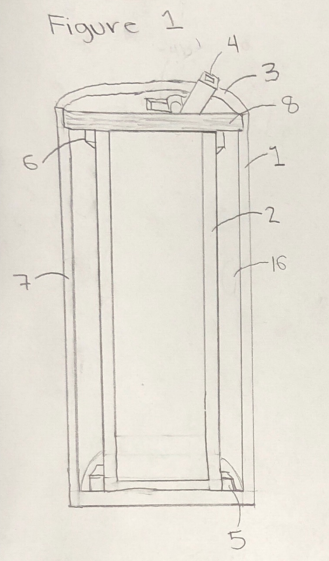
\includegraphics{Figure1.png}\\
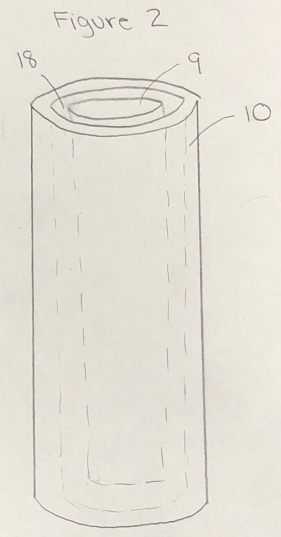
\includegraphics{Figure2.png}\\
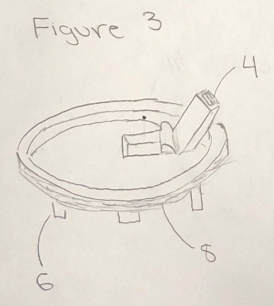
\includegraphics{Figure3.png}\\
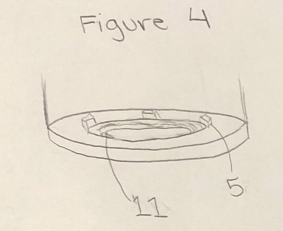
\includegraphics{Figure4.png}\\
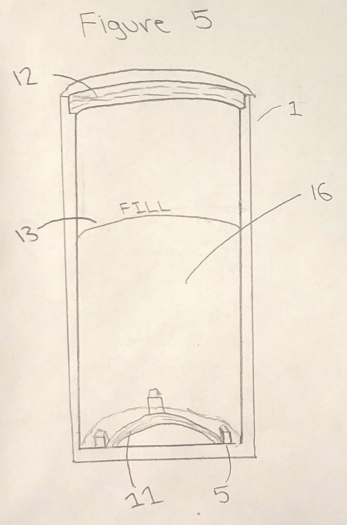
\includegraphics{Figure5.png}\\
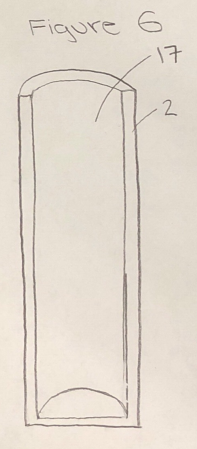
\includegraphics{Figure6.png}\\
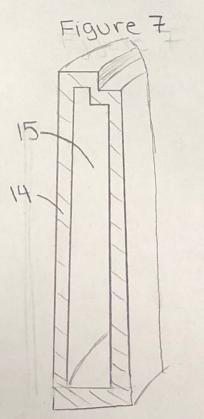
\includegraphics{Figure7.png}
\end{center}
\nocite{*}
\bibliographystyle{plain}
\bibliography{mybib.bib}
\end{document}